% Figure from MATH 591 notes, section 1. Compile with the notes preamble.
\begin{tikzpicture}[scale=0.9]
\draw[violet!75!black,thick] (0,0) circle (1);
\draw[teal!60!black,thick] (3,0) circle (1);
\draw[dashed,gray!70] (0,0) -- (3,0);
\fill (0,0) circle (1.5pt) node[font=\footnotesize,below left]{$p$};
\fill (3,0) circle (1.5pt) node[font=\footnotesize,below right]{$q$};
\node[font=\footnotesize,above] at (1.5,0.06) {$d(p,q)$};
\draw[|<->|,gray!70] (1,-0.6) -- (2,-0.6);
\node[font=\footnotesize,below] at (1.5,-1.12) {gap $=\tfrac13 d(p,q)$};
\node[violet!75!black,font=\footnotesize] at (-0.78,0.86) {$U$};
\node[teal!60!black,font=\footnotesize] at (3.8,0.86) {$V$};
\node[font=\footnotesize] at (1.5,1.42) {radii $r=\tfrac13 d(p,q)$};
\end{tikzpicture}
